\section{Quantity and quality}
\begin{definition}[Harmonic interval]
    Distance between two notes played \emph{simulatenously}.
\end{definition}

\begin{definition}[Melodic interval]
    Distance between two notes played \emph{one after the other}.
\end{definition}

\begin{definition}[Interval quantity]
    The number of notes on the diatonic scale (consecutive unaltered different pitches) from the starting note to the end note.
\end{definition}

\begin{definition}[Simple intervals]
    Intervals with a quantity less than an octave.
\end{definition}

\begin{definition}[Compound intervals]
    Intervals with a quantity higher than an octave.
\end{definition}

If we talk about \emph{simple intervals}, we have some predefined quantities. Each of them has some accepted \textbf{qualities}:

\begin{center}
    \begin{tabular}{r|l}
        \textbf{Quantity} & Compatible \textbf{quantities} \\
        \hline
        Unison & Perfect \\
        Second & Major, minor \\
        Third & Major, minor \\
        Fourth & Perfect, augmented, diminished \\
        Fifth & Perfect, augmented, diminished \\
        Sixth & Major, minor \\
        Seventh & Major, minor \\
        Octave & Perfect
    \end{tabular}
\end{center}

\subsection{Multiple augmentation / diminution}
An interval can be altered through additions of subtractions of half tones.

\begin{figure}
    \begin{center}
        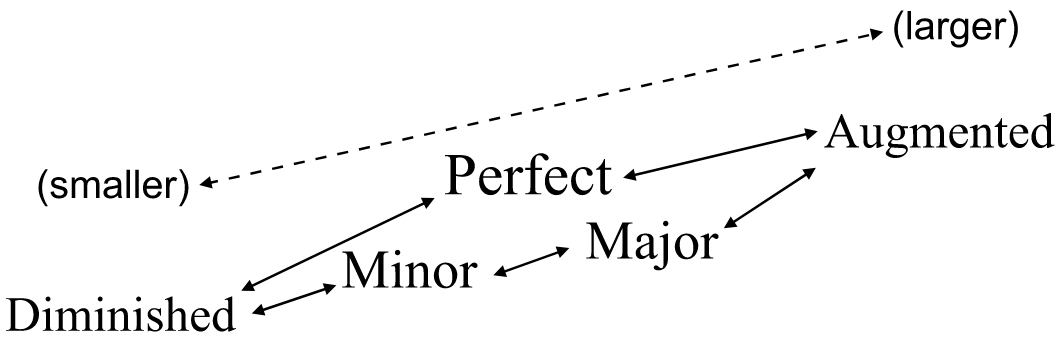
\includegraphics[width=0.8\textwidth]{img/quality}
        \caption{Interval quality chart}
    \end{center}
\end{figure}

In music notation, this is usually carried out through sharps and flats (or double sharps and double flats). From these accidentals we gather augmented / diminished intervals, but also double augmented and double augmented intervals\footnote{It is theoretically possible to reach a maximum quantity of a \emph{quintuply augmented fourth} (or \emph{quintuply diminished fifth}) by altering a tritone through a double flat - double sharp pair.}. In practice,  double augmented / double diminished intervals are rare in music, not to mention more altered quantities.

\subsection{Tritone}
Both between fifths and fourths there is a \emph{single} interval which is characterized by a much harsher sound than the others: while the others are \emph{consonant} that one is \emph{dissonant}. This interval is called the \textbf{tritone}.

\begin{definition}[Tritone]
    An augmented fourth / diminished fifth (which is always between F and B and always made up of 6 half tones or 3 whole tones - hence the name).
\end{definition}

This interval is also popularly called the \emph{diabolus in musica}, because it is the only dissonant exception to the consonant set of fourths and fifths.

Moreover, the tritone \emph{is half the width of an octave}.

\subsection{Compound intervals}
Compound intervals can be obtained by adding a 7th to an existing simple interval. Therefore, a two-octave interval is a 15th.

\subsection{Diatonic interval}
There is also a more vague type of interval, the \textbf{diatonic interval}, which essentially means: \emph{go from this note to the next one in the current diatonic scale}.

\begin{definition}[Diatonic interval]
    The distance between one note and another in the context of a specific diatonic scale.
\end{definition}

\section{Interval inversion}
An \textbf{interval inversion} can be performed by inverting the relative position of two notes, while keeping the pitch classes constant (this can be done through a single-note octave transposition).

\begin{figure}
    \begin{center}
        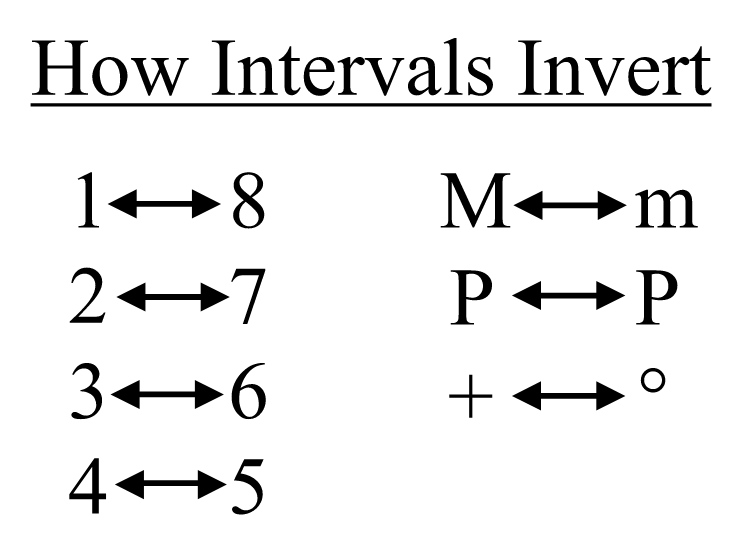
\includegraphics[width=0.4\textwidth]{img/inversion}
        \caption{Interval inversion chart}
    \end{center}
\end{figure}

As we can see, the sum of an interval quantity with the quantity of its inverted counterpart is always 9. Moreover:
\begin{itemize}
    \item Perfect intervals invert to perfect intervals.
    \item Augmented invervals invert to diminished intervals.
    \item Major intervals invert to minor intervals.
\end{itemize}